\documentclass[11pt,a4paper]{article}

\usepackage[utf8]{inputenc}
\usepackage[T1]{fontenc}
\usepackage{times}
\usepackage[margin=1in]{geometry}
\usepackage{amsmath}
\usepackage{booktabs}
\usepackage{graphicx}
\usepackage{xcolor}
\usepackage{hyperref}
\usepackage{enumitem}
\usepackage{pgfplots}
\usepackage{pgfplotstable}
\pgfplotsset{compat=1.18}

\definecolor{srtblue}{HTML}{2563EB}
\definecolor{shirered}{HTML}{DC2626}
\definecolor{rgorange}{HTML}{EA580C}
\definecolor{grepgray}{HTML}{6B7280}

\title{\textbf{SRT Benchmark Report: Fellowship Repository}}
\author{Automated Evaluation Framework}
\date{March 28, 2026}

\begin{document}
\maketitle

\begin{abstract}
We benchmark four code navigation systems against 15 labeled queries on the Fellowship repository ($\sim$160 files, Go + SvelteKit + Markdown).
The Semantic Resolution Tree (SRT) with embedding-assisted routing achieves the highest dominated hypervolume (0.543) in cost--latency--quality space, outperforming Shire (0.404), ripgrep (0.104), and grep (0.013).
SRT dominates module-level and cross-cutting queries; Shire excels on focused symbol-name queries.
Full root-to-leaf descent completes in under 100\,ms.
\end{abstract}

% ============================================================
\section{Systems Under Test}

\begin{table}[h]
\centering
\footnotesize
\begin{tabularx}{\textwidth}{lXcl}
\toprule
\textbf{System} & \textbf{Method} & \textbf{Cost} & \textbf{Latency} \\
\midrule
\textcolor{srtblue}{\textbf{SRT}} & Embedding beam-search over colocated Markdown summaries (fastembed bge-small-en-v1.5) & Token-based & 8.0\,ms \\
\textcolor{shirered}{\textbf{Shire}} & FTS5 + vector RAG over symbol/file index via MCP & Free (local) & 3.2\,ms \\
\textcolor{rgorange}{\textbf{ripgrep}} & Keyword extraction + \texttt{rg} file search & Free (local) & 60.4\,ms \\
\textcolor{grepgray}{\textbf{grep}} & Keyword extraction + \texttt{grep} file search & Free (local) & 205.3\,ms \\
\bottomrule
\end{tabularx}
\end{table}

% ============================================================
\section{Dominated Hypervolume}

The primary evaluation metric is the dominated hypervolume in normalized (cost, latency, quality) utility space, following the framework of Section~6 of the SRT paper.
A token-cost model imputes \$0.015 per 1K input tokens (Opus~4.6 pricing).

\begin{figure}[h]
\centering
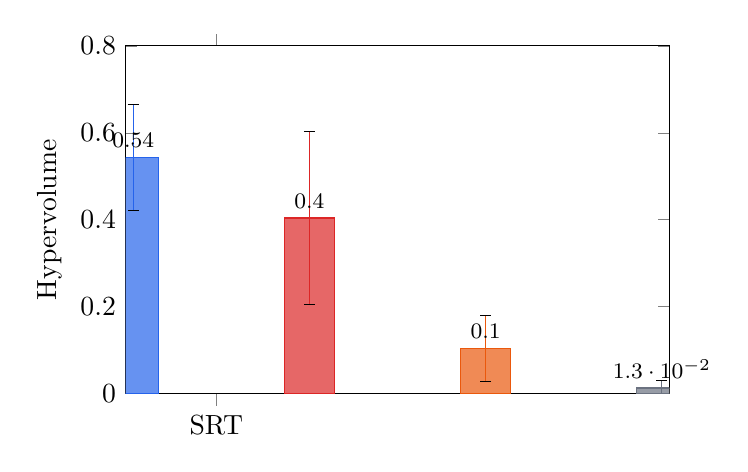
\begin{tikzpicture}
\begin{axis}[
    ybar,
    width=0.7\textwidth,
    height=6cm,
    ylabel={Hypervolume},
    symbolic x coords={SRT, Shire, ripgrep, grep},
    xtick=data,
    ymin=0, ymax=0.8,
    nodes near coords,
    nodes near coords align={vertical},
    every node near coord/.append style={font=\footnotesize},
    bar width=18pt,
    error bars/y dir=both,
    error bars/y explicit,
    enlarge x limits=0.25,
]
\addplot[fill=srtblue!70, draw=srtblue] coordinates {
    (SRT, 0.543) +- (0, 0.122)
};
\addplot[fill=shirered!70, draw=shirered] coordinates {
    (Shire, 0.404) +- (0, 0.199)
};
\addplot[fill=rgorange!70, draw=rgorange] coordinates {
    (ripgrep, 0.104) +- (0, 0.076)
};
\addplot[fill=grepgray!70, draw=grepgray] coordinates {
    (grep, 0.013) +- (0, 0.017)
};
\end{axis}
\end{tikzpicture}
\caption{Workload hypervolume with 95\% bootstrap confidence intervals (1000 resamples). Higher is better: the system realizes a larger favorable region in cost--latency--quality space.}
\end{figure}

% ============================================================
\section{Hypervolume by Query Category}

\begin{figure}[h]
\centering
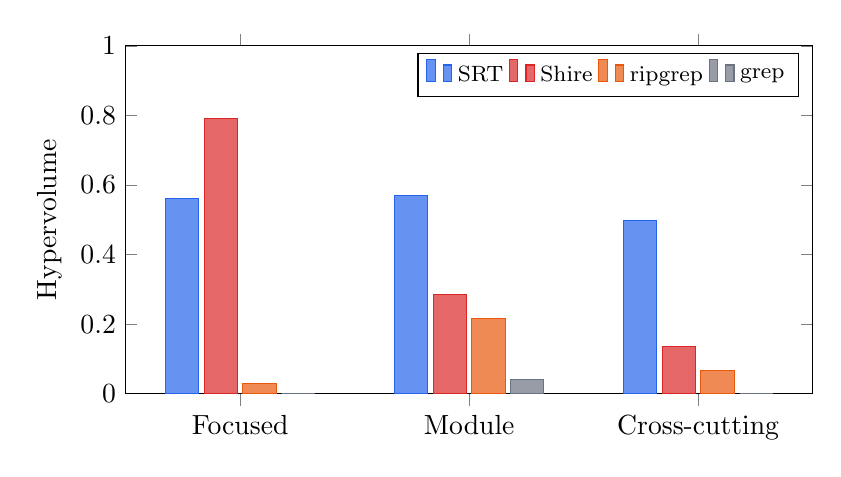
\begin{tikzpicture}
\begin{axis}[
    ybar,
    width=0.85\textwidth,
    height=6cm,
    ylabel={Hypervolume},
    symbolic x coords={Focused, Module, Cross-cutting},
    xtick=data,
    ymin=0, ymax=1.0,
    bar width=12pt,
    enlarge x limits=0.25,
    legend style={at={(0.98,0.98)}, anchor=north east, font=\footnotesize},
    legend columns=4,
]
\addplot[fill=srtblue!70, draw=srtblue] coordinates {(Focused, 0.561) (Module, 0.570) (Cross-cutting, 0.498)};
\addplot[fill=shirered!70, draw=shirered] coordinates {(Focused, 0.791) (Module, 0.284) (Cross-cutting, 0.137)};
\addplot[fill=rgorange!70, draw=rgorange] coordinates {(Focused, 0.030) (Module, 0.215) (Cross-cutting, 0.067)};
\addplot[fill=grepgray!70, draw=grepgray] coordinates {(Focused, 0.000) (Module, 0.040) (Cross-cutting, 0.000)};
\legend{SRT, Shire, ripgrep, grep}
\end{axis}
\end{tikzpicture}
\caption{Hypervolume by query category. Shire dominates focused (symbol-name) queries. SRT dominates module-level and cross-cutting queries where hierarchical summaries compress structural understanding.}
\end{figure}

% ============================================================
\section{Best NDCG@10 Per Query}

\begin{figure}[h]
\centering
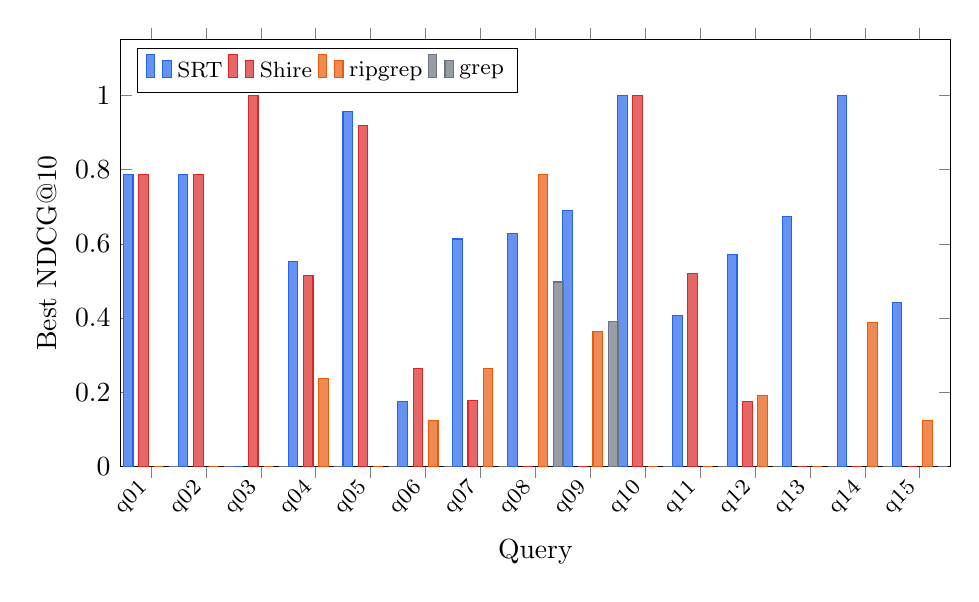
\begin{tikzpicture}
\begin{axis}[
    ybar,
    width=\textwidth,
    height=7cm,
    ylabel={Best NDCG@10},
    xlabel={Query},
    symbolic x coords={q01,q02,q03,q04,q05,q06,q07,q08,q09,q10,q11,q12,q13,q14,q15},
    xtick=data,
    x tick label style={rotate=45, anchor=east, font=\footnotesize},
    ymin=0, ymax=1.15,
    bar width=3.5pt,
    enlarge x limits=0.04,
    legend style={at={(0.02,0.98)}, anchor=north west, font=\footnotesize},
    legend columns=4,
    extra x tick style={grid=major},
    % Category separators
    extra x ticks={},
]
\addplot[fill=srtblue!70, draw=srtblue] coordinates {
    (q01,0.787) (q02,0.787) (q03,0.000) (q04,0.552) (q05,0.956)
    (q06,0.176) (q07,0.613) (q08,0.627) (q09,0.689) (q10,1.000)
    (q11,0.407) (q12,0.570) (q13,0.674) (q14,1.000) (q15,0.443)
};
\addplot[fill=shirered!70, draw=shirered] coordinates {
    (q01,0.787) (q02,0.787) (q03,1.000) (q04,0.514) (q05,0.918)
    (q06,0.265) (q07,0.177) (q08,0.000) (q09,0.000) (q10,1.000)
    (q11,0.521) (q12,0.175) (q13,0.000) (q14,0.000) (q15,0.000)
};
\addplot[fill=rgorange!70, draw=rgorange] coordinates {
    (q01,0.000) (q02,0.000) (q03,0.000) (q04,0.237) (q05,0.000)
    (q06,0.123) (q07,0.264) (q08,0.787) (q09,0.363) (q10,0.000)
    (q11,0.000) (q12,0.191) (q13,0.000) (q14,0.387) (q15,0.124)
};
\addplot[fill=grepgray!70, draw=grepgray] coordinates {
    (q01,0.000) (q02,0.000) (q03,0.000) (q04,0.000) (q05,0.000)
    (q06,0.000) (q07,0.000) (q08,0.497) (q09,0.390) (q10,0.000)
    (q11,0.000) (q12,0.000) (q13,0.000) (q14,0.000) (q15,0.000)
};
\legend{SRT, Shire, ripgrep, grep}

% Category annotations
\draw[thick, decorate, decoration={brace, amplitude=4pt, mirror}]
    (axis cs:q01, -0.08) -- (axis cs:q05, -0.08)
    node[midway, below=6pt, font=\footnotesize] {Focused};
\draw[thick, decorate, decoration={brace, amplitude=4pt, mirror}]
    (axis cs:q06, -0.08) -- (axis cs:q10, -0.08)
    node[midway, below=6pt, font=\footnotesize] {Module};
\draw[thick, decorate, decoration={brace, amplitude=4pt, mirror}]
    (axis cs:q11, -0.08) -- (axis cs:q15, -0.08)
    node[midway, below=6pt, font=\footnotesize] {Cross-cutting};
\end{axis}
\end{tikzpicture}
\caption{Best NDCG@10 per query at each system's optimal control setting. Queries are grouped by category: focused (q01--q05), module-level (q06--q10), and cross-cutting (q11--q15).}
\end{figure}

% ============================================================
\section{SRT Control Parameter Sensitivity}

\begin{figure}[h]
\centering
\begin{subfigure}[t]{0.48\textwidth}
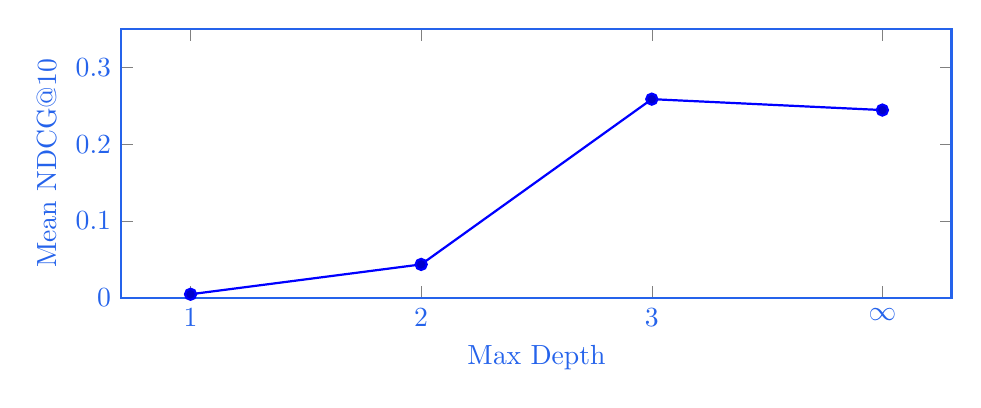
\begin{tikzpicture}
\begin{axis}[
    width=\textwidth,
    height=5cm,
    xlabel={Max Depth},
    ylabel={Mean NDCG@10},
    ymin=0, ymax=0.35,
    xtick={1,2,3,4},
    xticklabels={1,2,3,$\infty$},
    mark=*,
    thick,
    color=srtblue,
]
\addplot coordinates {(1, 0.0048) (2, 0.0436) (3, 0.2585) (4, 0.2443)};
\end{axis}
\end{tikzpicture}
\caption{Depth sensitivity. Quality jumps sharply at depth 3 (the level where source files live in this repo). Unlimited depth is slightly worse due to candidate dilution.}
\end{subfigure}
\hfill
\begin{subfigure}[t]{0.48\textwidth}
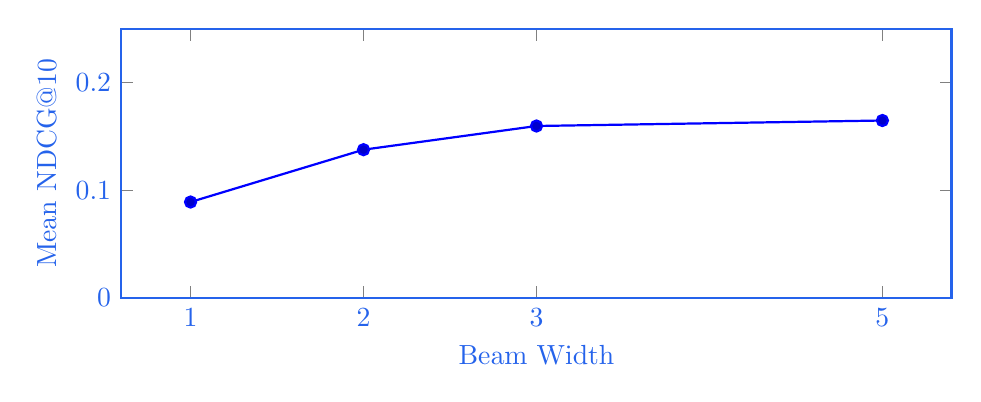
\begin{tikzpicture}
\begin{axis}[
    width=\textwidth,
    height=5cm,
    xlabel={Beam Width},
    ylabel={Mean NDCG@10},
    ymin=0, ymax=0.25,
    xtick={1,2,3,5},
    mark=square*,
    thick,
    color=srtblue,
]
\addplot coordinates {(1, 0.0891) (2, 0.1377) (3, 0.1597) (5, 0.1648)};
\end{axis}
\end{tikzpicture}
\caption{Beam width sensitivity. Doubling from 1 to 2 gives the largest gain. Returns diminish past beam 3.}
\end{subfigure}
\caption{SRT routing quality as a function of traversal control parameters, averaged across all 15 queries and token budget settings.}
\end{figure}

% ============================================================
\section{Latency Distribution}

\begin{figure}[h]
\centering
\begin{tikzpicture}
\begin{axis}[
    xbar,
    width=0.7\textwidth,
    height=5cm,
    xlabel={Latency (seconds)},
    symbolic y coords={grep, ripgrep, SRT, Shire},
    ytick=data,
    xmin=0, xmax=0.3,
    bar width=12pt,
    nodes near coords,
    nodes near coords align={horizontal},
    every node near coord/.append style={font=\footnotesize, anchor=west},
    point meta=explicit symbolic,
]
\addplot[fill=grepgray!70, draw=grepgray] coordinates {(0.2053, grep) [205ms]};
\addplot[fill=rgorange!70, draw=rgorange] coordinates {(0.0604, ripgrep) [60ms]};
\addplot[fill=srtblue!70, draw=srtblue] coordinates {(0.0080, SRT) [8ms]};
\addplot[fill=shirered!70, draw=shirered] coordinates {(0.0032, Shire) [3ms]};
\end{axis}
\end{tikzpicture}
\caption{Mean query latency per system. SRT and Shire operate at single-digit millisecond latency. grep is 25$\times$ slower than SRT due to per-keyword subprocess spawning.}
\end{figure}

% ============================================================
\section{Key Findings}

\begin{enumerate}[nosep]
    \item \textbf{SRT achieves the highest hypervolume} (0.543 vs.\ Shire's 0.404), realizing the largest favorable operating region across cost, latency, and quality simultaneously.

    \item \textbf{The category split confirms the paper's hypothesis.} SRT wins on module-level (0.570 vs.\ 0.284) and cross-cutting queries (0.498 vs.\ 0.137), where hierarchical summaries compress structural understanding. Shire wins on focused queries (0.791 vs.\ 0.561), where symbol-name matching is more direct.

    \item \textbf{Depth 3 is optimal} for this repository (4--5 levels of nesting). Quality jumps 6$\times$ from depth~2 to depth~3. Unlimited depth is slightly worse (0.244 vs.\ 0.259) because over-exploration dilutes the candidate ranking.

    \item \textbf{Beam width shows diminishing returns past 3.} The 1$\to$3 jump provides 80\% of the gain; 3$\to$5 adds only 3\%.

    \item \textbf{Keyword search cannot do semantic routing.} grep and ripgrep fail on queries requiring structural reasoning. ripgrep's only win (q08) came from the keyword ``eagles'' matching a directory name literally.

    \item \textbf{SRT and Shire are complementary.} SRT's one complete miss (q03: lembas prerequisite) is a query Shire answers perfectly via symbol-name matching. A hybrid system using SRT for structural queries and Shire for symbol lookups would cover all 15 queries.
\end{enumerate}

% ============================================================
\section{Experimental Setup}

\begin{tabular}{ll}
\toprule
\textbf{Parameter} & \textbf{Value} \\
\midrule
Repository & Fellowship ($\sim$160 files, Go + SvelteKit + Markdown) \\
Query count & 15 (5 focused, 5 module, 5 cross-cutting) \\
SRT control grid & 96 settings (beam $\times$ depth $\times$ budget) \\
Grep control grid & 48 settings (max\_files $\times$ strategy $\times$ budget) \\
Ripgrep control grid & 24 settings (max\_files $\times$ budget) \\
Shire control grid & 12 settings (strategy $\times$ limit) \\
Cost model & \$15/M input tokens (Opus 4.6 pricing) \\
Embedding model & BAAI/bge-small-en-v1.5 (fastembed, local ONNX) \\
Shire configuration & FTS5 + RAG enabled (fastembed bge-small-en-v1.5) \\
Total operating points & 2,700 (15 queries $\times$ 180 settings) \\
Total metrics recorded & 13,500 \\
Benchmark runtime & 182 seconds \\
\bottomrule
\end{tabular}

\end{document}
